\chapter{\DivisionByNineSectionName}
\label{sec:divisionbynine}

\RU{Простая функция:}\EN{A very simple function:}

\begin{lstlisting}
int f(int a)
{
	return a/9;
};
\end{lstlisting}

% sections:

\EN{
\subsection{x86}

\subsubsection{MSVC}

Here is what we get after compiling with MSVC 2010:

\lstinputlisting{patterns/04_scanf/1_simple/ex1_MSVC_EN.asm}

\TT{x} is a local variable.

According to the \CCpp standard it must be visible only in this function and not from any other external scope. 
Traditionally, local variables are stored on the stack. 
There are probably other ways to allocate them, but in x86 that is the way it is.

\myindex{x86!\Instructions!PUSH}
The goal of the instruction following the function prologue, \TT{PUSH ECX}, is not to save the \ECX state 
(notice the absence of corresponding \TT{POP ECX} at the function's end).

In fact it allocates 4 bytes on the stack for storing the \TT{x} variable.

\label{stack_frame}
\myindex{\Stack!Stack frame}
\myindex{x86!\Registers!EBP}
\TT{x} is to be accessed with the assistance of the \TT{\_x\$} macro (it equals to -4) and the \EBP register pointing to the current frame.

Over the span of the function's execution, \EBP is pointing to the current \gls{stack frame}
making it possible to access local variables and function arguments via \TT{EBP+offset}.

\myindex{x86!\Registers!ESP}
It is also possible to use \ESP for the same purpose, although that is not very convenient since it changes frequently.
The value of the \EBP could be perceived as a \IT{frozen state} of the value in \ESP at the start of the function's execution.

% FIXME1 это уже было в 02_stack?
Here is a typical \gls{stack frame} layout in 32-bit environment:

\begin{center}
\begin{tabular}{ | l | l | }
\hline
\dots & \dots \\
\hline
EBP-8 & local variable \#2, \MarkedInIDAAs{} \TT{var\_8} \\
\hline
EBP-4 & local variable \#1, \MarkedInIDAAs{} \TT{var\_4} \\
\hline
EBP & saved value of \EBP \\
\hline
EBP+4 & return address \\
\hline
EBP+8 & \argument \#1, \MarkedInIDAAs{} \TT{arg\_0} \\
\hline
EBP+0xC & \argument \#2, \MarkedInIDAAs{} \TT{arg\_4} \\
\hline
EBP+0x10 & \argument \#3, \MarkedInIDAAs{} \TT{arg\_8} \\
\hline
\dots & \dots \\
\hline
\end{tabular}
\end{center}

The \scanf function in our example has two arguments.

The first one is a pointer to the string containing \TT{\%d} and the second is the address of the \TT{x} variable.

\myindex{x86!\Instructions!LEA}
First, the \TT{x} variable's address is loaded into the \EAX register by the \TT{lea eax, DWORD PTR \_x\$[ebp]} instruction.

\LEA stands for \IT{load effective address}, and is often used for forming an address ~(\myref{sec:LEA}).

We could say that in this case \LEA simply stores the sum of the \EBP register value and the \TT{\_x\$} macro in the \EAX register.

This is the same as \INS{lea eax, [ebp-4]}.

So, 4 is being subtracted from the \EBP register value and the result is loaded in the \EAX register.
Next the \EAX register value is pushed into the stack and \scanf is being called.

\printf is being called after that with its first argument --- a pointer to the string:
\TT{You entered \%d...\textbackslash{}n}.

The second argument is prepared with: \TT{mov ecx, [ebp-4]}.
The instruction stores the \TT{x} variable value and not its address, in the \ECX register.

Next the value in the \ECX is stored on the stack and the last \printf is being called.

\clearpage
\subsection{MSVC + \olly}
\index{\olly}

\RU{Попробуем этот же пример в}\EN{Let's try this example in} \olly.
\RU{Загружаем, нажимаем F8 (\stepover) до тех пор, пока не окажемся в своем исполняемом файле,
а не в}\EN{Let's load it and keep pressing F8 (\stepover) until we reach our executable file
instead of} \TT{ntdll.dll}.
\RU{Прокручиваем вверх до тех пор, пока не найдем \main}\EN{Scroll up until \main appears}.
\RU{Щелкаем на первой инструкции (\TT{PUSH EBP}), нажимаем F2 (\IT{set a breakpoint}), 
затем F9 (\IT{Run}) и точка останова срабатывает на начале \main.}
\EN{Click on the first instruction (\TT{PUSH EBP}), press F2 (\IT{set a breakpoint}), 
then F9 (\IT{Run}).
The breakpoint will be triggered when \main begins.}

\RU{Трассируем до того места, где готовится адрес переменной $x$}%
\EN{Let's trace to the point where the address of the variable $x$ is calculated}:

\begin{figure}[H]
\centering
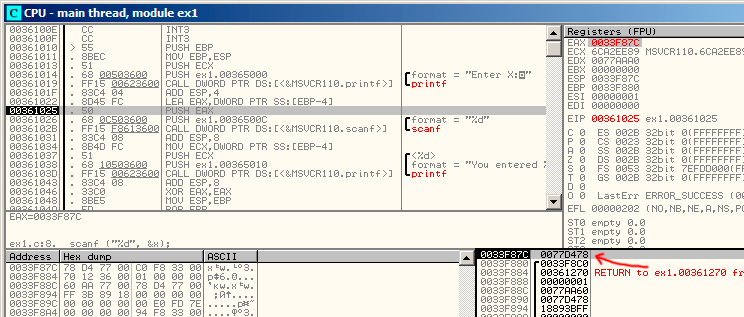
\includegraphics[scale=\FigScale]{patterns/04_scanf/1_simple/ex1_olly_1.png}
\caption{\olly: \RU{вычисляется адрес локальной переменной}\EN{The address of the local variable is calculated}}
\label{fig:scanf_ex1_olly_1}
\end{figure}

\RU{На \EAX в окне регистров можно нажать правой кнопкой и далее выбрать}
\EN{Right-click the \EAX in the registers window and then select} \q{Follow in stack}.
\RU{Этот адрес покажется в окне стека.}
\EN{This address will appear in the stack window.}
\RU{Смотрите, это переменная в локальном стеке. Я нарисовал там красную стрелку}\EN{The red arrow, I have added, points to the variable in the local stack}.
\RU{И там сейчас какой-то мусор}\EN{At that moment this location contains some garbage} (\TT{0x6E494714}).
\RU{Адрес этого элемента стека сейчас, при помощи \PUSH запишется в этот же стек рядом}%
\EN{Now with the help of \PUSH instruction the address of this stack element is going to be stored to the same stack on the next position}.
\RU{Трассируем при помощи F8 вплоть до конца исполнения \scanf}\EN{Let's trace with F8 until the \scanf execution completes}.
\RU{А пока \scanf исполняется, в консольном окне, вводим, например, 123}%
\EN{During the \scanf execution, we input, for example, 123, in the console window}:

\begin{figure}[H]
\centering
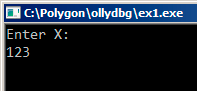
\includegraphics[scale=\NormalScale]{patterns/04_scanf/1_simple/ex1_olly_2.png}
\caption{\RU{Ввод пользователя в консольном окне}\EN{User input in the console window}}
\label{fig:scanf_ex1_olly_2}
\end{figure}

\clearpage
\RU{Вот тут }\scanf \RU{отработал}\EN{completed its execution already}:

\begin{figure}[H]
\centering
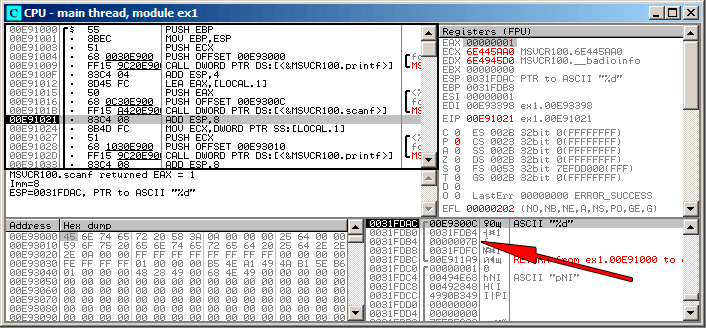
\includegraphics[scale=\FigScale]{patterns/04_scanf/1_simple/ex1_olly_3.png}
\caption{\olly: \scanf \RU{исполнилась}\EN{executed}}
\label{fig:scanf_ex1_olly_3}
\end{figure}

\scanf \RU{вернул}\EN{returns} $1$ \InENRU \EAX, \RU{что означает, что он успешно прочитал одно 
значение}\EN{which implies that it has read successfully one value}.
\RU{В наблюдаемом нами элементе стека теперь}\EN{If we look again at the stack element corresponding to the local variable it now contains} \TT{0x7B} (123).

\clearpage
\RU{Чуть позже это значение копируется из стека в регистр \ECX и передается в \printf}
\EN{Later this value is copied from the stack to the \ECX register and passed to \printf}:

\begin{figure}[H]
\centering
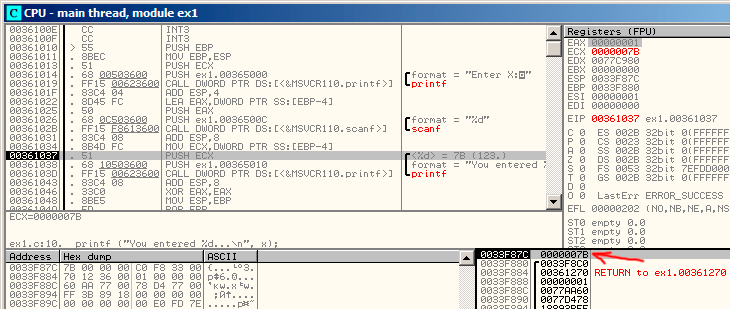
\includegraphics[scale=\FigScale]{patterns/04_scanf/1_simple/ex1_olly_4.png}
\caption{\olly: \RU{готовим значение для передачи в}\EN{preparing the value for passing to} \printf}
\label{fig:scanf_ex1_olly_4}
\end{figure}


\subsubsection{GCC}

Let's try to compile this code in GCC 4.4.1 under Linux:

\lstinputlisting{patterns/04_scanf/1_simple/ex1_GCC.asm}

\myindex{puts() instead of printf()}
GCC replaced the \printf call with call to \puts. The reason for this was explained in ~(\myref{puts}).

% TODO: rewrite
%\RU{Почему \scanf переименовали в \TT{\_\_\_isoc99\_scanf}, я честно говоря, пока не знаю.}
%\EN{Why \scanf is renamed to \TT{\_\_\_isoc99\_scanf}, I do not know yet.}
% 
% Apparently it has to do with the ISO c99 standard compliance. By default GCC allows specifying a standard to adhere to.
% For example if you compile with -std=c89 the outputted assmebly file will contain scanf and not __isoc99__scanf. I guess current GCC version adhares to c99 by default.
% According to my understanding the two implementations differ in the set of suported modifyers (See printf man page)

As in the MSVC example---the arguments are placed on the stack using the \MOV instruction.

\subsubsection{By the way}

By the way, this simple example is a demonstration of the fact that compiler translates
list of expressions in \CCpp-block into sequential list of instructions.
There are nothing between expressions in \CCpp, and so in resulting machine code, 
there are nothing between, control flow slips from one expression to the next one.


\subsection{ARM}

\subsubsection{\OptimizingKeilVI (\ThumbMode)}

\lstinputlisting[caption=\OptimizingKeilVI (\ThumbMode)]{patterns/15_structs/4_packing/packing_Keil_thumb.asm}

As we may recall, here a structure is passed instead of pointer to one,
and since the first 4 function arguments in ARM are passed via registers,
the structure's fields are passed via \TT{R0-R3}.

\myindex{ARM!\Instructions!LDRB}
\myindex{x86!\Instructions!MOVSX}
\TT{LDRB} loads one byte from memory and extends it to 32-bit, taking its sign into account.
This is similar to \MOVSX in x86.
Here it is used to load fields $a$ and $c$ from the structure.

\myindex{Function epilogue}

One more thing we spot easily is that instead of function epilogue, there is jump to another function's epilogue!
Indeed, that was quite different function, not related in any way to ours, however, it has exactly
the same epilogue 
(probably because, it hold 5 local variables too 
($5*4=0x14$)).

Also it is located nearby (take a look at the addresses).

Indeed, it doesn't matter which epilogue gets executed,
if it works just as we need.

Apparently, Keil decides to reuse a part of another function to economize.

The epilogue takes 4 bytes while jump~---only 2.

\subsubsection{ARM + \OptimizingXcodeIV (\ThumbTwoMode)}

\lstinputlisting[caption=\OptimizingXcodeIV (\ThumbTwoMode)]{patterns/15_structs/4_packing/packing_Xcode_thumb.asm}

\myindex{ARM!\Instructions!SXTB}
\myindex{x86!\Instructions!MOVSX}
\TT{SXTB} (\IT{Signed Extend Byte}) is analogous to \MOVSX in x86.
All the rest~---just the same.


\subsectionold{MIPS}

\lstinputlisting[caption=\Optimizing GCC 4.4.5 (IDA)]{patterns/12_FPU/2_passing_floats/MIPS_O3_IDA_EN.lst}

And again, we see here \INS{LUI} loading a 32-bit part of a \Tdouble number into \$V0.
And again, it's hard to comprehend why.

\myindex{MIPS!\Instructions!MFC1}

The new instruction for us here is \INS{MFC1} (\q{Move From Coprocessor 1}).
The FPU is coprocessor number 1, hence \q{1} in the instruction name.
This instruction transfers values from the coprocessor's registers to the registers of the CPU (\ac{GPR}).
So in the end the result from \TT{pow()} is moved to registers \$A3 and \$A2, 
and \printf takes a 64-bit double value from this register pair.


\subsection{How it works}

That's how division can be replaced by multiplication and division with $2^{n}$ numbers:

\[
	result = 
	\frac{input}{divisor} = 
	\frac{input \cdot \frac{2^{n}}{divisor}}{2^{n}} = 
	\frac{input \cdot M}{2^{n}}
\]

Where $M$ is a \IT{magic} coefficient.

This is how $M$ can be computed:

\[
	M = \frac{2^{n}}{divisor}
\]

So these code snippets usually have this form:

\[
	result = \frac{input \cdot M}{2^{n}}
\]

%
Division by $2^{n}$ is usually done by simply shifting to the right.

If $n<32$, then the low part of the \gls{product} is shifted (in \EAX or \RAX).

$n$ is chosen in order to minimize the error.

When doing signed division, the sign of the multiplication result is also added to the output result.

Take a look at the difference:

\begin{lstlisting}
int f3_32_signed(int a)
{
	return a/3;
};

unsigned int f3_32_unsigned(unsigned int a)
{
	return a/3;
};
\end{lstlisting}

In the unsigned version of the function, the \IT{magic} coefficient is \TT{0xAAAAAAAB} 
and the multiplication result is divided by $2^{33}$.

In the signed version of the function, the \IT{magic} coefficient is \TT{0x55555556} 
and the multiplication result is divided by $2^{32}$.
There are no division instruction though: the result is just taken from \EDX. 

The sign is also taken from the multiplication result: the high 32 bits of the result are shifted by 31
(leaving the sign in the least significant bit of \EAX).
1 is added to the final result if the sign is negative, for result correction.

\lstinputlisting[caption=\Optimizing MSVC 2012]{\CURPATH/2_EN.asm}

\subsubsection{More theory}

It works, because that is how it's possible to replace division by multiplication:

\[
	\frac{x}{c} = x\frac{1}{c}
\]

$\frac{1}{c}$ is called \IT{multiplicative inverse} and can be precomputed by compiler.

But this is for real numbers
What about integers?
It's possible to find \IT{multiplicative inverse} for integer in the environment of modulo arithmetics

\footnote{\href{http://go.yurichev.com/17359}{Wikipedia}}.
\ac{CPU} registers fits nicely: each is limited by 32 or 64 bits, so almost any arithmetic operation on registers are in fact
opeartions on modulo $2^{32}$ or $2^{64}$.

Read more about it in [\HenryWarren 10-3].

\subsection{Getting the divisor}

\subsubsection{Variant \#1}

Often, the code looks like this:

\lstinputlisting{\CURPATH/form_EN.asm}

Let's denote the 32-bit \IT{magic} coefficient as $M$, the shifting coefficient as $C$ and the divisor as $D$.

The divisor we need to get is:

\[
D=\frac{2^{32 + C}}{M}
\]

For example:

\lstinputlisting[caption=\Optimizing MSVC 2012]{\CURPATH/ex1.asm}

This is:

\[
D=\frac{2^{32 + 3}}{2021161081}
\]

\myindex{Wolfram Mathematica}

The numbers are larger than 32-bit, so we can use Wolfram Mathematica for convenience:

\begin{lstlisting}[caption=Wolfram Mathematica]
In[1]:=N[2^(32+3)/2021161081]
Out[1]:=17.
\end{lstlisting}

So the divisor from the code we used as example is 17.

For x64 division, things 
are the same, but $2^{64}$ has to be used instead of $2^{32}$:

\begin{lstlisting}
uint64_t f1234(uint64_t a)
{
	return a/1234;
};
\end{lstlisting}

\begin{lstlisting}[caption=\Optimizing MSVC 2012 x64]
f1234	PROC
	mov	rax, 7653754429286296943		; 6a37991a23aead6fH
	mul	rcx
	shr	rdx, 9
	mov	rax, rdx
	ret	0
f1234	ENDP
\end{lstlisting}

\begin{lstlisting}[caption=Wolfram Mathematica]
In[1]:=N[2^(64+9)/16^^6a37991a23aead6f]
Out[1]:=1234.
\end{lstlisting}

\subsubsection{Variant \#2}

A variant with omitted arithmetic shift also exist:

\begin{lstlisting}
		mov     eax, 55555556h ; 1431655766
		imul    ecx
		mov     eax, edx
		shr     eax, 1Fh
\end{lstlisting}

The method of getting divisor is simplified:

\[
D=\frac{2^{32}}{M}
\]

As of my example, this is:

\[
D=\frac{2^{32}}{1431655766}
\]

\myindex{Wolfram Mathematica}

And again we use Wolfram Mathematica:

\begin{lstlisting}[caption=Wolfram Mathematica]
In[1]:=N[2^32/16^^55555556]
Out[1]:=3.
\end{lstlisting}

The divisor is 3.

\input{\CURPATH/exercises_EN.tex}
}
\RU{
\subsubsection{x86}

\myparagraph{\NonOptimizing MSVC}

Имеем в итоге (MSVC 2010):

\lstinputlisting[caption=MSVC 2010]{patterns/14_bitfields/2_set_reset/set_reset_msvc.asm}

\myindex{x86!\Instructions!OR}
Инструкция \OR здесь устанавливает в переменной ещё один бит, игнорируя остальные.

\myindex{x86!\Instructions!AND}
А \AND сбрасывает некий бит. Можно также сказать, что \AND здесь копирует все биты, кроме одного. 
Действительно, во втором операнде \AND выставлены в единицу те биты, которые нужно сохранить, 
кроме одного, копировать который мы не хотим (и который 0 в битовой маске).
Так проще понять и запомнить.

\clearpage
\mysubparagraph{\olly}

Попробуем этот пример в \olly.
Сначала, посмотрим на двоичное представление используемых нами констант:

\TT{0x200} (0b0000000000000000000{\color{red}1}000000000) (т.е. 10-й бит (считая с первого)).

Инвертированное \TT{0x200} это \TT{0xFFFFFDFF} (0b1111111111111111111{\color{red}0}111111111).

\TT{0x4000} (0b00000000000000{\color{red}1}00000000000000) (т.е. 15-й бит).

Входное значение это: \TT{0x12340678} (0b10010001101000000011001111000).
Видим, как оно загрузилось:

\begin{figure}[H]
\centering
\myincludegraphics{patterns/14_bitfields/2_set_reset/olly1.png}
\caption{\olly: значение загружено в \ECX}
\label{fig:set_reset_olly1}
\end{figure}

\clearpage
\OR исполнилась:

\begin{figure}[H]
\centering
\myincludegraphics{patterns/14_bitfields/2_set_reset/olly2.png}
\caption{\olly: \OR сработал}
\label{fig:set_reset_olly2}
\end{figure}

15-й бит выставлен: \TT{0x1234{\color{red}4}678} 
(0b10010001101000{\color{red}1}00011001111000).

\clearpage
Значение перезагружается снова (потому что использовался режим компилятора без оптимизации): 

\begin{figure}[H]
\centering
\myincludegraphics{patterns/14_bitfields/2_set_reset/olly3.png}
\caption{\olly: значение перезагрузилось в \EDX}
\label{fig:set_reset_olly3}
\end{figure}

\clearpage
\AND исполнилась:

\begin{figure}[H]
\centering
\myincludegraphics{patterns/14_bitfields/2_set_reset/olly4.png}
\caption{\olly: \AND сработал}
\label{fig:set_reset_olly4}
\end{figure}

10-й бит очищен (или, иным языком, оставлены все биты кроме 10-го) и итоговое значение это \\
\TT{0x12344{\color{red}4}78} (0b1001000110100010001{\color{red}0}001111000).

\myparagraph{\Optimizing MSVC}

Если скомпилировать в MSVC с оптимизацией (\Ox), то код еще короче:

\lstinputlisting[caption=\Optimizing MSVC]{patterns/14_bitfields/2_set_reset/set_reset_msvc_Ox.asm}

\myparagraph{\NonOptimizing GCC}

Попробуем GCC 4.4.1 без оптимизации:

\lstinputlisting[caption=\NonOptimizing GCC]{patterns/14_bitfields/2_set_reset/set_reset_gcc.asm}

Также избыточный код, хотя короче, чем у MSVC без оптимизации.

Попробуем теперь GCC с оптимизацией \Othree:

\myparagraph{\Optimizing GCC}

\lstinputlisting[caption=\Optimizing GCC]{patterns/14_bitfields/2_set_reset/set_reset_gcc_O3.asm}

Уже короче. Важно отметить, что через регистр \AH компилятор работает с частью регистра \EAX. 
Это его часть от 8-го до 15-го бита включительно.

\RegTableOne{RAX}{EAX}{AX}{AH}{AL}

\myindex{Intel!8086}
\myindex{Intel!80386}
N.B. В 16-битном процессоре 8086 аккумулятор имел название \AX 
и состоял из двух 8-битных половин~--- \AL (младшая часть) и \AH (старшая). 
В 80386 регистры были расширены до 32-бит, 
аккумулятор стал называться \EAX, но в целях совместимости, к его \IT{более старым} частям всё ещё можно 
обращаться как к \AX/\AH/\AL.

Из-за того, что все x86 процессоры~--- наследники 16-битного 8086, эти \IT{старые} 16-битные опкоды короче 
нежели более новые 32-битные. 
Поэтому инструкция \INS{or ah, 40h} занимает только 3 байта. 
Было бы логичнее сгенерировать здесь \INS{or eax, 04000h}, но это уже 5 байт, или даже 6 
(если регистр в первом операнде не \EAX).

\myparagraph{\Optimizing GCC и regparm}

Если мы скомпилируем этот же пример не только с включенной оптимизацией \Othree, 
но ещё и с опцией \TT{regparm=3}, о которой я писал немного выше, то получится ещё короче:

\lstinputlisting[caption=\Optimizing GCC]{patterns/14_bitfields/2_set_reset/set_reset_gcc_O3_regparm3.asm}

\myindex{Inline code}
Действительно~--- первый аргумент уже загружен в \EAX, и прямо здесь можно начинать с ним работать. 
Интересно, что и пролог функции (\INS{push ebp / mov ebp,esp}) и эпилог (\INS{pop ebp}) 
функции можно смело выкинуть за ненадобностью, 
но возможно GCC ещё не так хорош для подобных оптимизаций по размеру кода. 
Впрочем, в реальной жизни подобные короткие функции лучше всего автоматически делать в виде 
\IT{inline-функций} (\myref{inline_code}).


\subsubsection{ARM}

\myparagraph{\OptimizingKeilVI (\ThumbMode)}

\lstinputlisting{patterns/04_scanf/1_simple/ARM_IDA.lst}

\myindex{\CLanguageElements!\Pointers}
Чтобы \scanf мог вернуть значение, ему нужно передать указатель на переменную типа \Tint.
\Tint~--- 32-битное значение, для его хранения нужно только 4 байта, и оно помещается в 32-битный регистр.

\myindex{IDA!var\_?}
Место для локальной переменной \GTT{x} выделяется в стеке, \IDA наименовала её \IT{var\_8}. 
Впрочем, место для неё выделять не обязательно, т.к. \glslink{stack pointer}{указатель стека} \ac{SP} уже указывает на место, 
свободное для использования.
Так что значение указателя \ac{SP} копируется в регистр \Reg{1}, и вместе с format-строкой, 
передается в \scanf.

\myindex{ARM!\Instructions!LDR}
Позже, при помощи инструкции \INS{LDR}, это значение перемещается из стека в регистр \Reg{1}, чтобы быть переданным в \printf.

\myparagraph{ARM64}

\lstinputlisting[caption=\NonOptimizing GCC 4.9.1 ARM64,numbers=left]{patterns/04_scanf/1_simple/ARM64_GCC491_O0_RU.s}

Под стековый фрейм выделяется 32 байта, что больше чем нужно. Может быть, это связано с выравниваем по границе памяти?
Самая интересная часть~--- это поиск места под переменную $x$ в стековом фрейме (строка 22).
Почему 28? Почему-то, компилятор решил расположить эту переменную в конце стекового фрейма, а не в начале.
Адрес потом передается в \scanf, которая просто сохраняет значение, введенное пользователем, в памяти по этому адресу.
Это 32-битное значение типа \Tint.
Значение загружается в строке 27 и затем передается в \printf.


\subsubsection{MIPS}

\myindex{MIPS!\Registers!FCCR}

В сопроцессоре MIPS есть бит результата, который устанавливается в FPU и проверяется в CPU.

Ранние MIPS имели только один бит (с названием FCC0), а у поздних их 8 (с названием FCC7-FCC0).
Этот бит (или биты) находятся в регистре с названием FCCR.

\lstinputlisting[caption=\Optimizing GCC 4.4.5 (IDA)]{patterns/12_FPU/3_comparison/MIPS_O3_IDA_RU.lst}

\myindex{MIPS!\Instructions!C.LT.D}
\INS{C.LT.D} сравнивает два значения. 
\GTT{LT} это условие \q{Less Than} (меньше чем).
\GTT{D} означает переменные типа \Tdouble.

В зависимости от результата сравнения, бит FCC0 устанавливается или очищается.

\myindex{MIPS!\Instructions!BC1T}
\myindex{MIPS!\Instructions!BC1F}
\INS{BC1T} проверяет бит FCC0 и делает переход, если бит выставлен.
\GTT{T} означает, что переход произойдет если бит выставлен (\q{True}).
Имеется также инструкция \INS{BC1F} которая сработает, если бит сброшен (\q{False}).

В зависимости от перехода один из аргументов функции помещается в регистр \$F0.


\subsection{Как это работает}

Вот как деление может быть заменено на умножение и деление на числа $2^{n}$:

\[
	result = 
	\frac{input}{divisor} = 
	\frac{input \cdot \frac{2^{n}}{divisor}}{2^{n}} = 
	\frac{input \cdot M}{2^{n}}
\]

Где $M$ это \IT{magic}-коэффициент.

Как вычислить $M$:

\[
	M = \frac{2^{n}}{divisor}
\]

Так что эти фрагменты кода обычно имеют форму:

\[
	result = \frac{input \cdot M}{2^{n}}
\]

Деление на $2^{n}$ производится обычным битовым сдвигом вправо.

Если $n\geq32$, то тогда сдвигается старшая часть \glslink{product}{произведения} (в \EDX или \RDX).

$n$ выбирается так, чтобы улучшить точность результата.

Если делать знаковое деление, знак результата умножения также добавляется к результату.

Посмотрите на разницу:

\begin{lstlisting}
int f3_32_signed(int a)
{
	return a/3;
};

unsigned int f3_32_unsigned(unsigned int a)
{
	return a/3;
};
\end{lstlisting}

В беззнаковой версии функции, \IT{magic}-коэффициент это \TT{0xAAAAAAAB} и результат умножения делится на $2^{33}$.

В знаковой версии функции, \IT{magic}-коэффициент это
 \TT{0x55555556} и результат умножения делится на $2^{32}$.
Впрочем здесь нет инструкции деления: результат просто берется из \EDX. 

Знак результата умножения также учитывается: старшие 32 бита результата сдвигаются на 31
(таким образом, оставляя знак в самом младшем бите \EAX).

1 прибавляется к конечному результату, если знак отрицательный, для коррекции результата.

\lstinputlisting[caption=\Optimizing MSVC 2012]{\CURPATH/2_RU.asm}

\subsubsection{Больше теории}

Это работает, потому что можно заменить деление на умножение вот так:

\[
	\frac{x}{c} = x\frac{1}{c}
\]


$\frac{1}{c}$ называется \IT{обратное число} и может быть предвычислено компилятором.

Но это для вещественных чисел.
Что насчет целых чисел?

Можно найти \IT{обратное число по модулю} для целого числа в среде модульной арифметики
\footnote{\href{http://go.yurichev.com/17359}{Wikipedia}}.

Регистры \ac{CPU} подходят идеально: каждый ограничен 32 или 64-ю битами, так что практически любая арифметическая операция над регистрами это на самом деле операции по модулю $2^{32}$ или $2^{64}$.

Читайте больше об этом в \InSqBrackets{\HenryWarren 10-3}.

\subsection{Определение делителя}

\subsubsection{Вариант \#1}

Часто, код имеет вид:

\lstinputlisting{\CURPATH/form_RU.asm}

Определим 32-битную \IT{magic}-коэффициент через $M$, коэффициент сдвига через $C$ и делитель через $D$.

Делитель, который нам нужен это:

\[
D=\frac{2^{32 + C}}{M}
\]

Например:

\lstinputlisting[caption=\Optimizing MSVC 2012]{\CURPATH/ex1.asm}

Это:

\[
D=\frac{2^{32 + 3}}{2021161081}
\]

\myindex{Wolfram Mathematica}
Числа больше чем 32-битные, так что мы можем использовать Wolfram Mathematica для удобства:

\begin{lstlisting}[caption=Wolfram Mathematica]
In[1]:=N[2^(32+3)/2021161081]
Out[1]:=17.
\end{lstlisting}

Так что искомый делитель это 17.

При делении в x64, всё то же самое, только нужно использовать $2^{64}$ вместо $2^{32}$:

\begin{lstlisting}
uint64_t f1234(uint64_t a)
{
	return a/1234;
};
\end{lstlisting}

\begin{lstlisting}[caption=\Optimizing MSVC 2012 x64]
f1234	PROC
	mov	rax, 7653754429286296943		; 6a37991a23aead6fH
	mul	rcx
	shr	rdx, 9
	mov	rax, rdx
	ret	0
f1234	ENDP
\end{lstlisting}

\begin{lstlisting}[caption=Wolfram Mathematica]
In[1]:=N[2^(64+9)/16^^6a37991a23aead6f]
Out[1]:=1234.
\end{lstlisting}

\subsubsection{Вариант \#2}

Бывает также вариант с пропущенным арифметическим сдвигом, например:

\begin{lstlisting}
		mov     eax, 55555556h ; 1431655766
		imul    ecx
		mov     eax, edx
		shr     eax, 1Fh
\end{lstlisting}

Метод определения делителя упрощается:

\[
D=\frac{2^{32}}{M}
\]

Для моего примера, это:

\[
D=\frac{2^{32}}{1431655766}
\]

\myindex{Wolfram Mathematica}
Снова используем Wolfram Mathematica:

\begin{lstlisting}[caption=Wolfram Mathematica]
In[1]:=N[2^32/16^^55555556]
Out[1]:=3.
\end{lstlisting}

Искомый делитель это 3.

\input{\CURPATH/exercises_RU.tex}
}

